\documentclass[18pt]{article}
\usepackage[utf8]{inputenc}
\usepackage[a4paper, tmargin=0.7in, bmargin=0.7in, lmargin=0.75in, rmargin=0.5in]{geometry}
\usepackage[nottoc,notlot,notlof]{tocbibind}
\usepackage[justification=centering]{caption}
\usepackage{graphicx}
\usepackage{wrapfig}
\usepackage[table]{xcolor}
\setlength{\tabcolsep}{18pt}
\renewcommand{\arraystretch}{1.5}
%\newcolumntype{s}{>{\columncolor[HTML]{AAACED}}{4cm} p{2cm}}
\newcolumntype{R}[1]{>{\raggedleft\arraybackslash}p{#1}}
\newcolumntype{L}[1]{>{\raggedright\arraybackslash}p{#1}}

% \usepackage{draftwatermark}
% \SetWatermarkText{
\includegraphics[width=0.6\textwidth]{default_apollo_logo.png}}
% \SetWatermarkLightness{0.2}
% \SetWatermarkScale{1}
\usepackage{background}
\backgroundsetup{contents=
\includegraphics{default_apollo_logo.png},scale=0.4,opacity=0.1,angle=0}

% \DeclareGraphicsExtensions{.png}
% \graphicspath{{figures}}

% \usepackage{appendix}
% \usepackage{multirow}
\usepackage{xcolor}
\usepackage{subcaption}
% \usepackage[autostyle]{csquotes}
\usepackage{hyperref}
\hypersetup{
    colorlinks=true,
    linkcolor=blue,
    citecolor=blue,      
    urlcolor=black,
}
\usepackage{soul}
\usepackage[english]{babel}
\usepackage{pdfpages}
\usepackage{fancyhdr}
\usepackage{hyperref}
\usepackage[yyyymmdd]{datetime}
\renewcommand{\dateseparator}{-}
\renewcommand{\headrulewidth}{0.4pt}
\renewcommand{\footrulewidth}{0.4pt}
\renewcommand{\familydefault}{\sfdefault}
\renewcommand{\baselinestretch}{1.5}
\pagestyle{fancy}
\fancyhead[L]{\today}
%\fancyhead[C]{Apollo Energy Analytics}
\fancyhead[C]{
\includegraphics[width=2cm]{default_apollo_logo.png}}
\fancyhead[R]{20221119APOLLO}
\fancyfoot[C]{\thepage}
\fancyfoot[L]{Helios IOT Systems Pvt. Ltd., Pune, MH, India}
\fancyfoot[R]{\href{mailto:contact@apolloenergyanalytics.com}{contact@apolloenergyanalytics.com}}
 

\title{Plant Performance Report}

\begin{document}

\vspace{0.5cm}
\centerline{\huge \textbf{Sample Plant Performance Report}}
\vspace{0.5cm}

{\large \hspace{-0.5cm}\textbf{Name:} Mr. Abhay Tilwankar \hfill \textbf{Plant:} ABC Plant \hfill \textbf{Location:} Karnataka, India}
\newline
{\large \hspace{-0.5cm}\textbf{DC Capacity:} X MWp \hfill \textbf{AC Capacity:} Y MW \hfill \textbf{COD:} 2013-09-04}


\noindent
{\color{red} \rule{\linewidth}{0.5mm}}
\vspace{0.5cm}

\begin{figure}[!h]
	\centering
	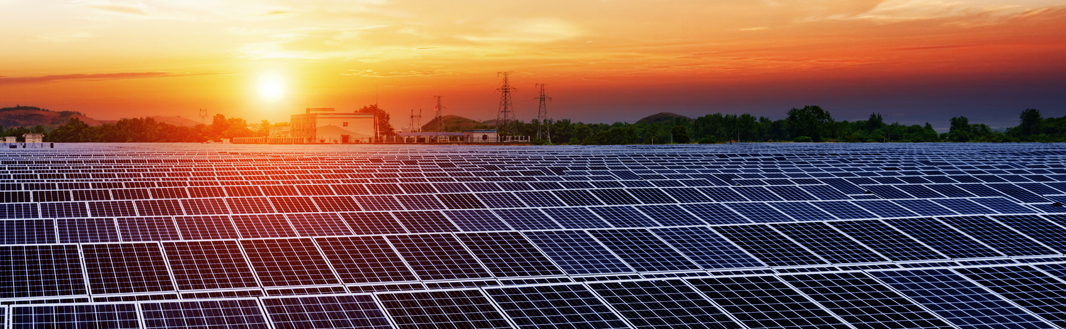
\includegraphics[width=\textwidth,height=0.25\textwidth]{poster.png}
	\caption*{}
	\label{fig:poster}
\end{figure}


\section*{Summary}
\hspace{0.5cm} The ABC Plant is located in Karnataka, India. This plant has X MWp (DC) and YMW (AC) capacity. This plant was commisioned in 2013-09-04. This report includes analysis of plant ABC from 1st October 2023 to 30th October 2023. The plant is performing {\color{green!55!blue}\hl {2\% higher }} compared to budgeted expectations. The plant-downtime in this period was {\color{green!55!blue}\hl {0\%}},  although few inverters are not woring on their full potentials which are described in section 4.2 of this report. This report includes plant level overall analysis to in depth equipment level analysis. 

\section{Budget vs Actual}

In the month of Oct,23 the plant has performed higher compared to expectations. This section compares major KPIs of plant which describes the overall health and performance of plant. These KPIs are performance ratio (PR), Generation (Net Export), Irradiance and Temperature.  Here budgeted values are taken from plant design document (PVSyst). 


\begin{center}
\begin{tabular} { |R{4cm}|L{2cm}|L{2cm}|L{2cm}| }
	\hline
	Parameter & Budgeted & Actual & Gain/Loss\\
	\hline
	Performance Ratio(\%) & 80\% & 81\% & \cellcolor{green}{1\%} \\
	Generation (MWh) & 2345 & 2392 & \cellcolor{green}{2\%} \\
	Irradiance (kW/m\textsuperscript{2}) & 169 & 168.15 & \cellcolor{red}{0.5\%} \\
	Temperatur (C) & 33.1 & 33 & \cellcolor{green}{0.2\%} \\
	\hline
\end{tabular}
\end{center}



\section{Loss Analysis}
 Here is the bird view of all the major KPIs for Oct, 23 period. 
 

 
\begin{figure}
	\centering
	\begin{subfigure}[b]{0.3\textwidth}
		\centering
		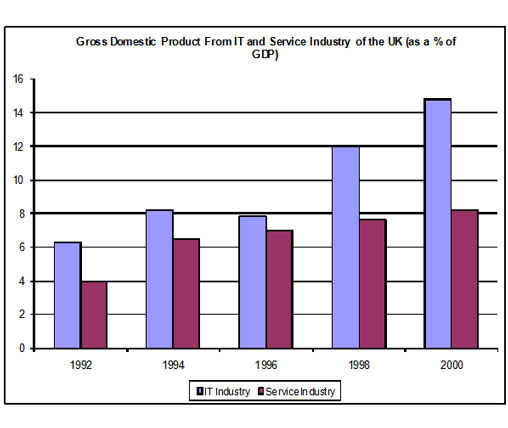
\includegraphics[width=\textwidth]{figures/sample1.jpeg}
		\caption{Generation}
		\label{fig:y equals x}
	\end{subfigure}
\hfill
	\begin{subfigure}[b]{0.3\textwidth}
	\centering
	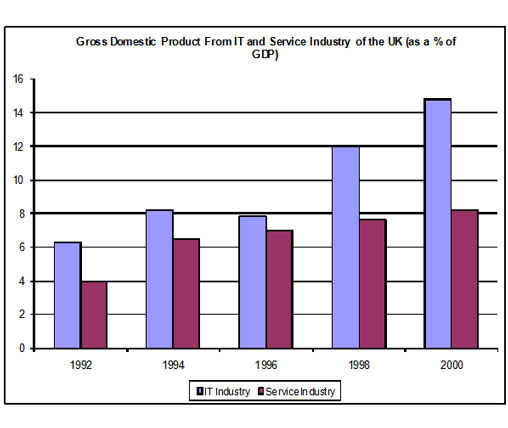
\includegraphics[width=\textwidth]{figures/sample1.jpeg}
	\caption{Performance Ratio}
	\label{fig:y equals x}
\end{subfigure}
\hfill
	\begin{subfigure}[b]{0.3\textwidth}
	\centering
	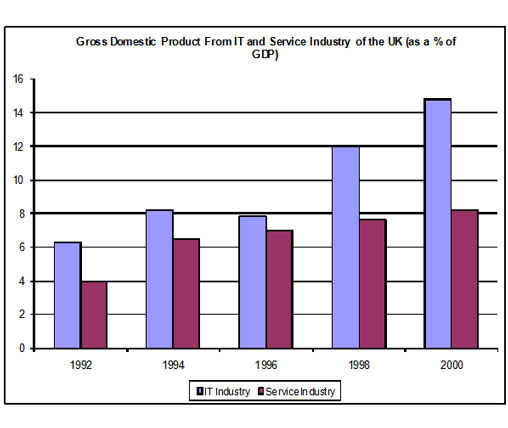
\includegraphics[width=\textwidth]{figures/sample1.jpeg}
	\caption{Irradiance}
	\label{fig:y equals x}
\end{subfigure}


\begin{subfigure}[b]{0.3\textwidth}
	\centering
	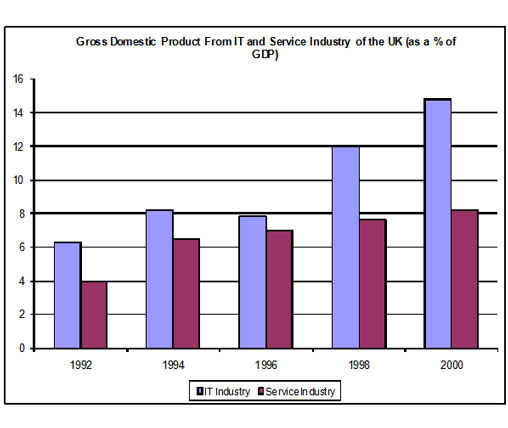
\includegraphics[width=\textwidth]{figures/sample1.jpeg}
	\caption{Plant Availability}
	\label{fig:y equals x}
\end{subfigure}
\hfill
\begin{subfigure}[b]{0.3\textwidth}
	\centering
	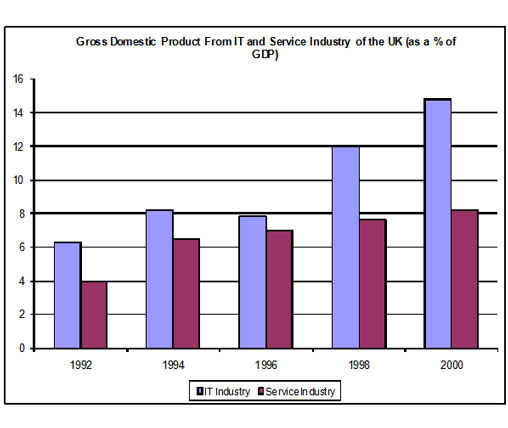
\includegraphics[width=\textwidth]{figures/sample1.jpeg}
	\caption{Grid Availability}
	\label{fig:y equals x}
\end{subfigure}
\hfill
\begin{subfigure}[b]{0.3\textwidth}
	\centering
	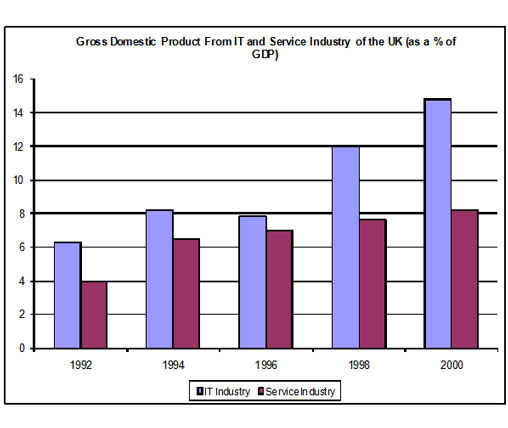
\includegraphics[width=\textwidth]{figures/sample1.jpeg}
	\caption{Capacity Utilization Factor}
	\label{fig:y equals x}
\end{subfigure}


\end{figure}


\section{Plant Level KPIs}

It is known fact that all losses which occures in solar PV plant are sequential loss hence we have represented them in the same sequence of occurance in form of waterfall diagram of loss. Here blue/green color shows the gain and red color shows the loss. It has included all the important losses such as : shadow loss, soiling loss, degradation loss, clipping loss, load shading/curtailment loss, inverter level loss, temperature loss and also includes plant availability and grid availability to give a complete idea on how the overall losses are spreaded. Here for this time period 48\% of total loss is recoverable. 

\begin{figure}
	\centering
	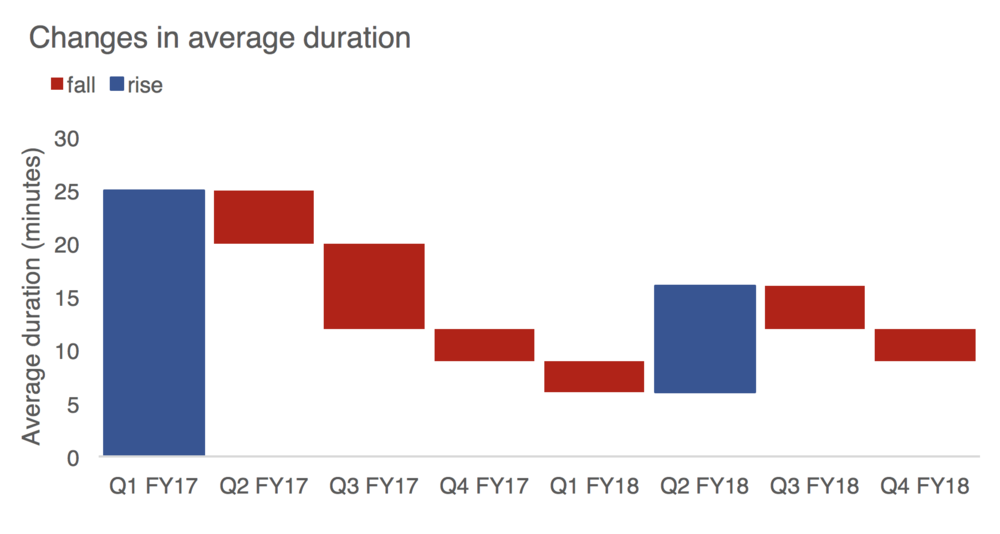
\includegraphics[width=12cm]{figures/loss_waterfall.png}
	\caption{Loss Waterfall}
	\label{fig: lw}
\end{figure}


\section{Asset Performance}

This sections deals with findings based on our detailed analysis using complex analytical layers. Here we have 3 subsections such as DC side, Inveretr and Transformer (AC Side). 

\subsection{DC side performance}

\subsection{Inverter Performance}

\subsection{Transformer Performance}

\end{document}